\def\web{WEB\xspace}
\def\WEB{WEB\xspace}

\chapter{WEB}
\setlength\columnsep{2.03em}

A common question on forums and lists, is in what language is \tex written in; the common  answer is that Knuth wrote \tex using  Pascal\footnote{See \protect\url{http://www.standardpascal.org/} for a list of currently supported Pascal versions.}. This is of course partly right as \text was written in \web and then translated automatically to Pascal. In the process \textit{literate programming} was discovered.

\web is a tool to implement the concept of ``literate programming''. Knuth’s original implementation will be in any respectable distribution of \TeX\, but the sources of the two tools (tangle and weave), together with a manual outlining the programming techniques, may be had from \texttt{CTAN}. Another common question is how to compile the original \tex sources. Although this is all unecessary as the  main distributions MikTeX and TeXLive do provide compiled sources for almost any conceivable machine, it is instructive when one is studying a subject to delve into its history and roots. This is the only way to get into the original author's mind and understand a system properly.

\texttt{Where to get the source code.} The source code is not in the normal distributions, you will need to get it from CTAN\footnote{\protect\url{http://mirror.ctan.org/systems/knuth/dist/web.zip}}. The file includes weave.web, \texttt{tangle.web}, \texttt{tangle.web} and the web manual in \file{tex} format. 


\texttt{Using \texttt{WEB}} The definite source for the manual, was written by Knuth in the form of a memo and if you have downloaded the code, you should be able to process it and read it. Knuth describes its purpose as:
\begin{quotation}
\noindent This memo describes how to write programs in the
\WEB language; and it also includes the full \WEB documentation for
\texttt{WEAVE} and \texttt{TANGLE}, the programs that read \WEB input and produce
\TeX\ and \texttt{PASCAL} output, respectively. The philosophy behind \texttt{WEB} is
that an experienced system programmer, who wants to provide the best
possible documentation of software products, needs two things
simultaneously:  a language like \TeX\ for formatting, and a language like
\texttt{PASCAL}  for programming. Neither type of language can provide the best
documentation by itself. But when both are appropriately combined, we
obtain a system that is much more useful than either language separately.
\end{quotation}

What it means, to understand the inner working of \tex you need to get profficient in three languages, Pascal, \tex and \web. It is not as daunting as it sounds for Pascal is almost readable as pseudocode and you are reading this book in order to learn a bit more about \tex. All in all a month's part-time work in evenings and weekends should get you going. If you are not on a Linux machine some extra time for setting everything up, might be required, but the executables are available in MikTeX as |.dlls| and executables |weave.exe| and |tangle.exe|\footnote{\url{YOUR DEFAULT PATH\textbackslash MiKTeX2.9\textbackslash miktex\textbackslash bin}}. To type code as \web all you need is a good text editor. All the processing will be done via |WEAVE| and then |TANGLE.|


\texttt{CWEB} The program |CWEB| is the successor to the |WEB|, it is available in all distributions and works as advertized both in |MiKTeX| as well as |TeXLive|. To try it out download a sample file or two from |CTAN|. I did download the example |wc.w|, note the extension is just |.w| and not |.web|, which has passed to history.  To run it use:

The main idea is to regard a program as a communication to human beings rather than as a set of instructions to a computer. Your program is also viewed as a hypertext document, rather like the World Wide Web. (Indeed, Knuth used the word WEB for this purpose long before CERN grabbed it!)

CWEB is a version of WEB for documenting C, C++, and Java programs. WEB was adapted to C by Silvio Levy in 1987, and since then both Knuth and Levy have revised and enhanced the system in many ways, notably to support C++ and ANSI C. Thus CWEB combines TeX with today's most widely used professional programming languages. You can get it by \url{ftp://ftp.cs.stanford.edu/pub/cweb/cweb.tar.gz}
\footnote{The CWEB System of Structured Documentation
by Donald E. Knuth and Silvio Levy (Reading, Massachusetts: Addison-Wesley, 1993), iv+227pp.
ISBN 0-201-57569-8}. See also Knuth's \url{http://www-cs-faculty.stanford.edu/~uno/cweb.html}

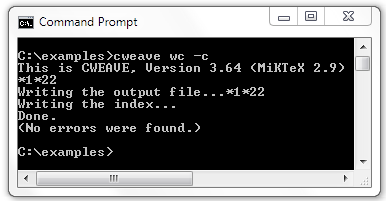
\includegraphics[width=10cm]{cweb01}

Version 3.61 of CWEB introduced cool new features with which you can weave programs in PDF format with clickable links, and these features have been refined in version 3.64. In fact, the new software gives you two ways to proceed, either with standard TeX together with Mark A. Wicks's program dvipdfm, or with an extension of TeX called pdfTeX. Instructions on how to use these features are explained in the current CWEB manual and examples appear in the Makefile.


processing the files with |CWEB| run without any trouble. The generated files include |wc.tex|, which can then be processed like any other |TeX| file. It runs without any errors using |pdfTeX|. Similarly the file was processed using |TANGLE| to generate the |C| source file.


\texttt{Literate programming.} Anyone that ever had the need to examine the code of a \alltex package can be thankful for the manner the code is documented, which although not using directly any of the \web related programs it provides literate programming. With literate programming the author of the program writes in a natural manner.

\texttt{Nuweb.} Nuweb can translate a single LP source into any number of code files in any mix of languages together with documentation in LaTeX. It does it in a single invocation; it does not have separate weave and tangle commands. It does not have the extensibility of noweb, but it can use the listings package of LaTeX to provide pretty-printing and the hyperref package to provide hyperlinks in PDF output. It also has extensive indexing and cross-referencing facilities including cross-references from the generated code back to the documentation, both as automatically generated comments and as strings that the code can use to report its behaviour. Vimes is a type-checker for Z notation which shows the use of nuweb in a practical application. Around 15,000 lines of nuweb source are translated into nearly 15,000 lines of |C/C++| code and over 460 pages of documentation. \footnote{\protect\url{http://sourceforge.net/projects/nuweb/}}. Nuweb is still actively maintained. 
\index{Literate programming! Nuweb}




%% based on a summary on http://www.tex.ac.uk/cgi-bin/texfaq2html?label=webpkgs